\input preamble.tex
\noindent
\section*{Industrielektronikk Øving 01 - En motstand}

I denne øvingen skal du bruke koblingsbrettet til å koble en motstand
til en spenningskilden på brettet. spenningskilden er en 230 AC til 24DC strømforsyning.   
\noindent \begin{center}
\begin{figure}[H]
\noindent \begin{centering}
%\includegraphics[angle=90,width=16cm]{\string"tegninger/Elektroteknikk - Breadboard\string".pdf}\vspace{2cm}
\par\end{centering}
\noindent \begin{centering}
%\includegraphics[width=16cm]{\string"tegninger/Elektroteknikk - koblingsbrett\string".jpg}
\par\end{centering}
$$\includegraphics[width=10cm]{./lIndustrielektronikk01.eps}$$
\end{figure}
\par\end{center}

\subsubsection*{Utstyr du trenger}
\begin{itemize}
\item Labbrettet
\item Rød og svart isolert ledning
\item Resistans på $3.3k\Omega$ 
\item Multimeter
\end{itemize}

\subsubsection*{Oppgaven}

Du skal koble en motstand $R_{1}=3.3k\Omega$ til en likespenningskilde
på 24VDC. På den oppkoblede kretsen skal du måle spenning over og strøm igjennom motstanden. 

\begin{enumerate}
\item Mål spenningen over motstanden $R_{1}$
\item Regn ut strømmen i kretsen
\item Koble inn et amperemeter og mål strømmen igjennom $R_{1}$ 
\item koble motstanden fra spenningskilden og mål resistansen $R_{1}$
\end{enumerate}

\subsubsection*{Innlevering}

Skriv en rapport for forsøket og lever på OneNote
\underbar{file ./lIndustrielektronikk01.tex}
\vskip 5pt 

\end{document}

